\documentclass[dvipsnames, tikz]{standalone}

% better text rendering
% https://tex.stackexchange.com/questions/664/why-should-i-use-usepackaget1fontenc
\newcommand{\usefonts}
{
  \usepackage[T1]{fontenc}
  \usepackage[utf8]{inputenc}
  \usepackage{microtype}
  \usepackage[l]{plex-serif}
  \usepackage{plex-mono}
}

% helpers
\newcommand{\subfigwidth}{0.49\linewidth}

\newcommand{\code}[1]{\lstinline{#1}}

\newcommand
{\captiondesc}
[1]
{
  \centering
  \vspace{0.5em}
  \parbox{0.8\linewidth}{\footnotesize{}#1}
}

\newcommand{\dd}[1]{\ensuremath{#1}}
\newcommand{\dddd}[2]{\ensuremath{\dd{#1},\,\dd{#2}}}

\newcommand{\dms}[3]{\ensuremath{\ang{#1}\,#2'\,#3''}}
\newcommand{\dmsdms}[6]{\ensuremath{\dms{#1}{#2}{#3},\,\dms{#4}{#5}{#6}}}
\usefonts{}

\usepackage{tikz}
\usetikzlibrary{positioning}

\begin{document}

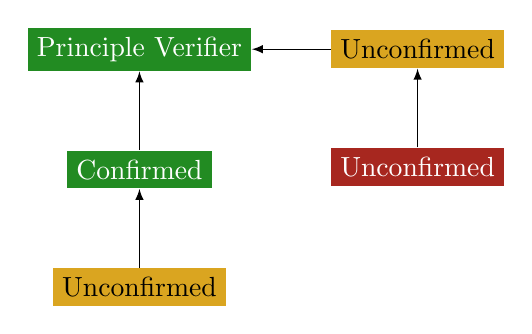
\begin{tikzpicture}
  [
    -latex,
    confirmed/.style={text=white, fill=ForestGreen},
    unconfirmed/.style={fill=Goldenrod},
    illegal/.style={text=white, fill=Mahogany}
  ]

  \node[confirmed] (pv) {Principle Verifier};
  \node[confirmed] (c) [below=of pv] {Confirmed};
  \node[unconfirmed] (uc1) [below=of c] {Unconfirmed};
  \node[unconfirmed] (uc2) [right=of pv] {Unconfirmed};
  \node[illegal] (i) [below=of uc2] {Unconfirmed};

  \draw (c) -- (pv);
  \draw (uc1) -- (c);
  \draw (uc2) -- (pv);
  \draw (i) -- (uc2);

\end{tikzpicture}

\end{document}
